\section{Base Finite Volume Schemes}\label{sec:basefv}

Our computational results use two different finite volume schemes
to update the cut cell mesh, to show that SRD can be used in a
variety of situations.
We will refer to these at the base schemes. 
The  base scheme is applied to the entire mesh, including  
to the small cut cells.  Since cut cells can have cell volumes that are
orders of magnitude smaller than the time step allowed by the full
cells, these will lead to instability without a stabilization algorithm.
SRD will be applied after each stage or step of the base scheme.

\begin{figure}
\begin{center}
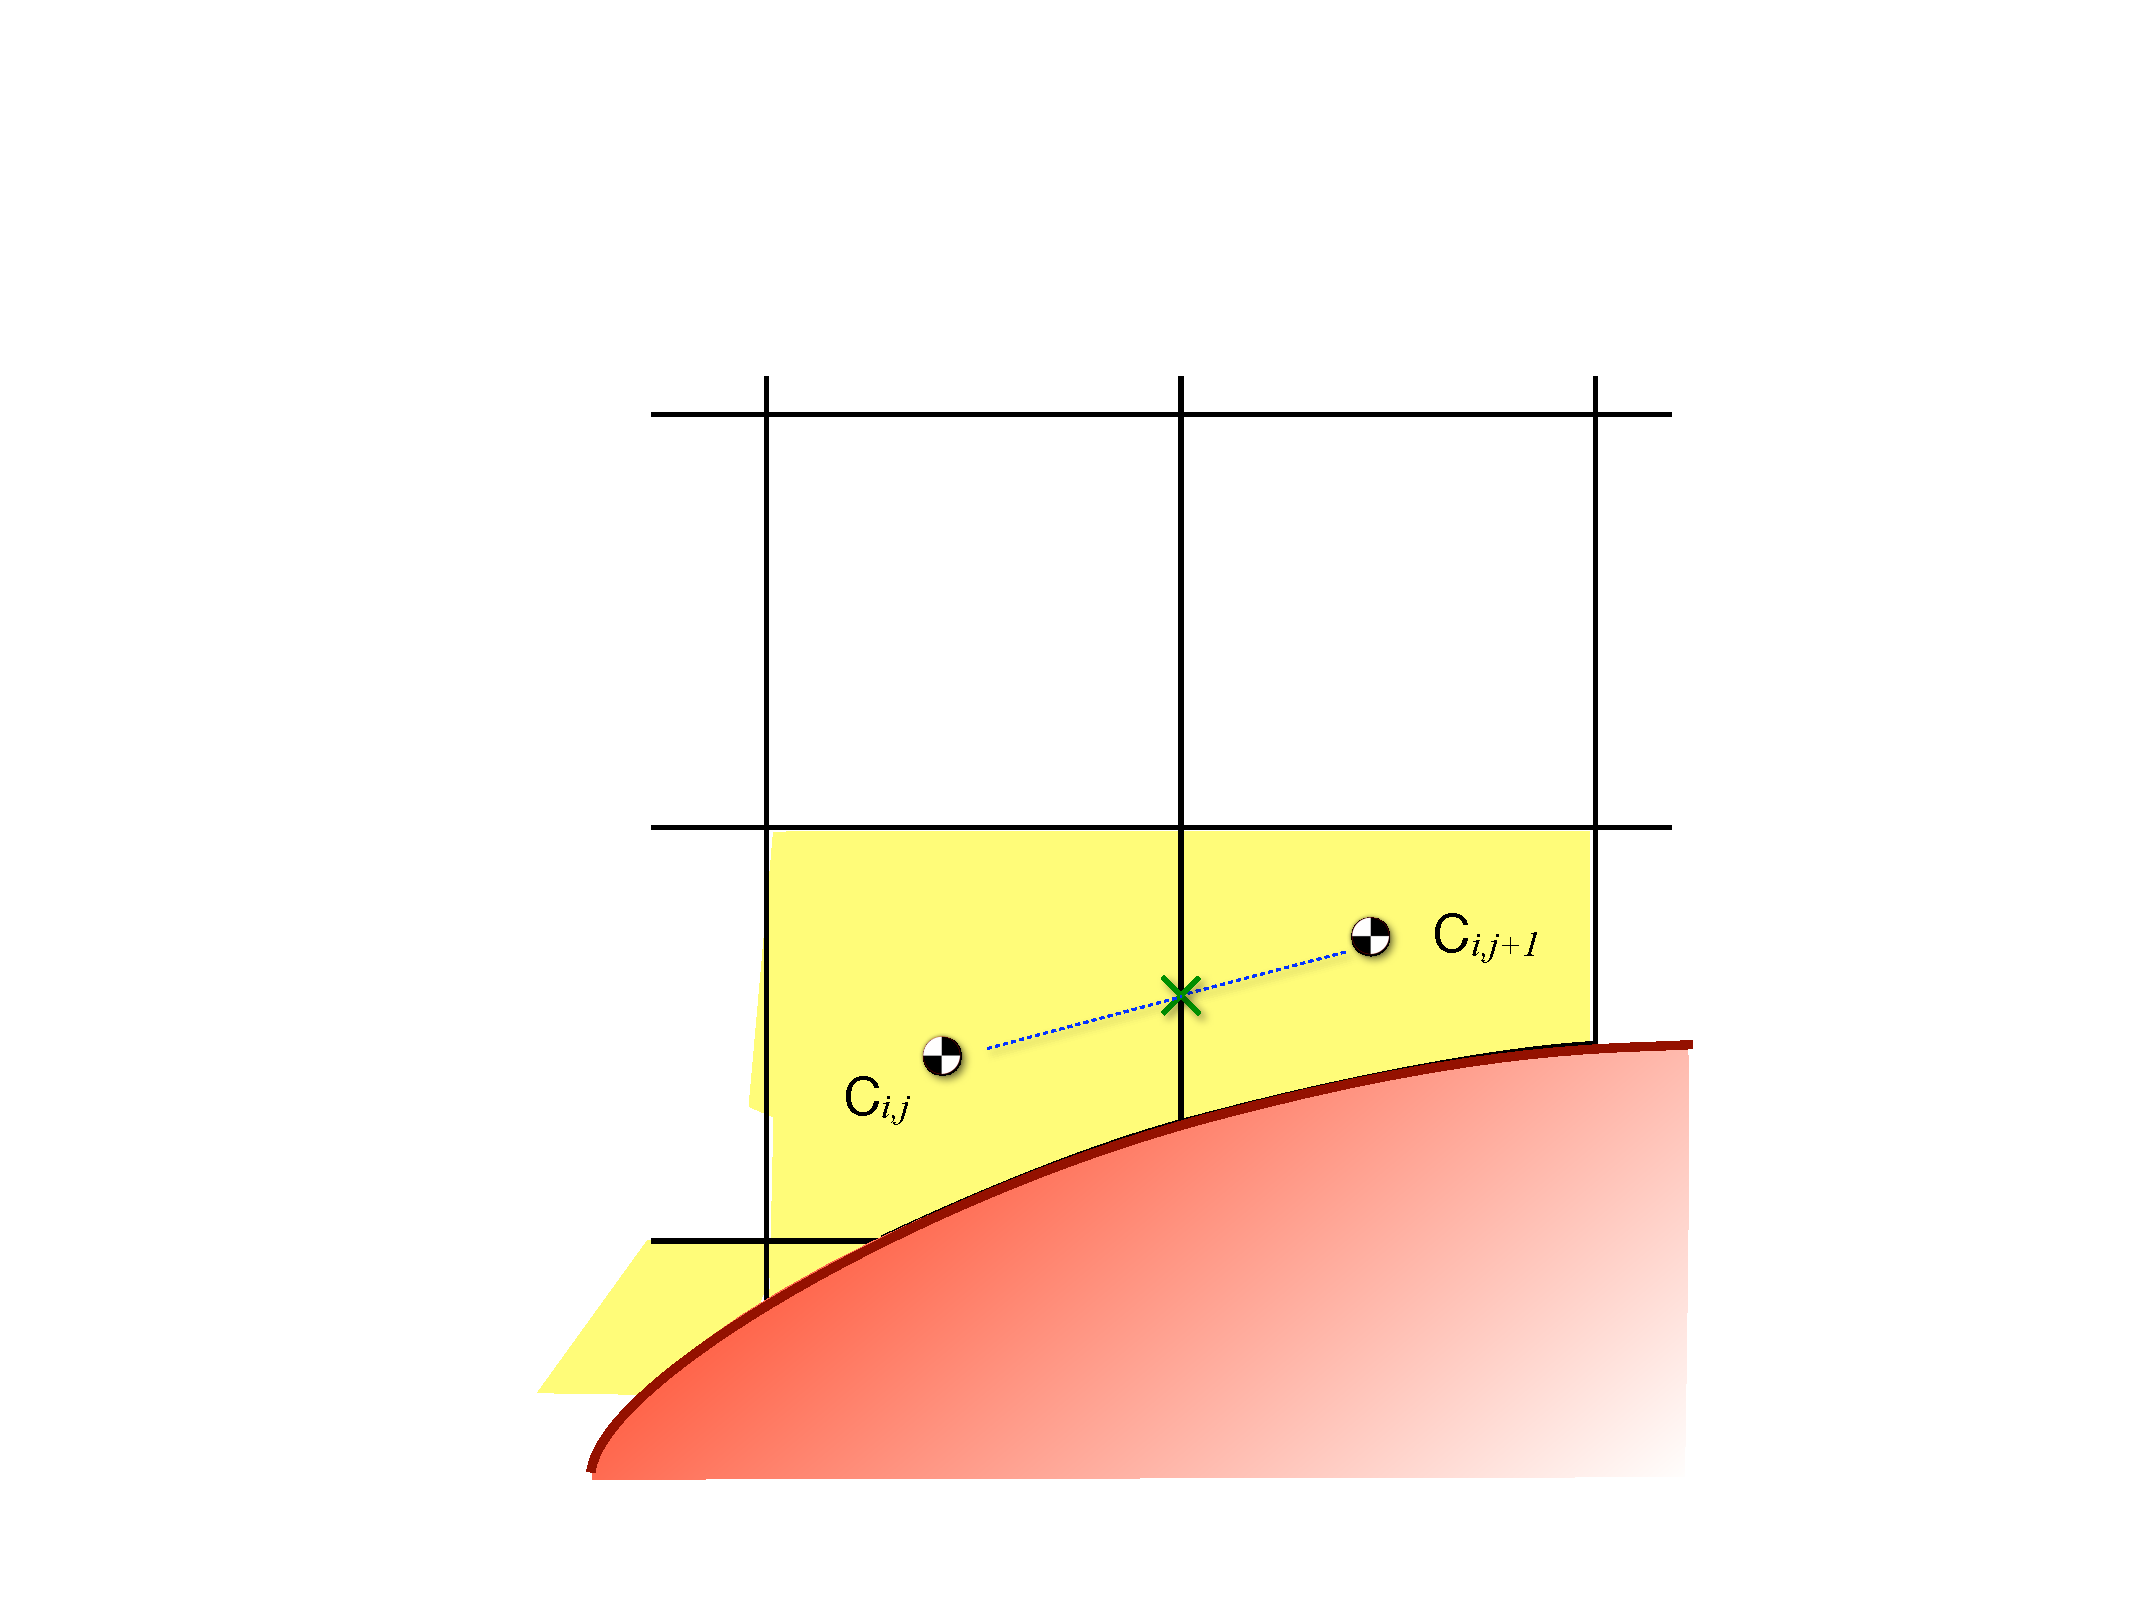
\includegraphics[width=3.2in]{figs/2dfig.pdf}
\caption{\sf Notation for mesh in two space dimensions. The cells shaded
in yellow are the cut cells.} 
\label{fig:2dfig}
\end{center}
\end{figure}

In both base schemes we sometimes use the LP-limiter \cite{May_Berger_LP} for the cut 
cells and one adjacent, to try to retain as much of the gradient as possible. 
 he LP limiter is much less diffusive than the alternative BJ limiter at cut cells,
although sometimes this is preferable. (AG - DESCRIBE MORE, INCLUDING BJ?)  We will always include which limiter is used
in the computational results.  Cells that are two away from a cut cell
can use any limiter. 

\subsection{Method of Lines approach}
The simplest scheme is to use a spatial discretization over the entire
mesh, and apply a Runge-Kutta scheme in time. This is a well-known
standard approach
on regular Cartesian meshes. It is adapted for the cut cells by
using a least squares reconstruction of the gradient that includes
either edge and node neighbors (the examples will always specify).
Limiting is done using the Barth-Jespersen limiter \cite{} 
on the cut cells and one adjacent neighbors. Any limiter
can be used for the regular cells.

The spatial reconstruction in the cut cells is no longer
coordinate-aligned, and need 
to include both $x$ and $y$ components of the gradient to 
reconstruct to the midpoint of the cell edge. This is indicated 
Figure \ref{fig:2dfig}  indicates this face location with a green $\times$.
The SRD stabilization scheme is applied after each stage of
the Runge-Kutta scheme. 
Note that the time step restriction that results from the von Neumann stability analysis of this scheme applied to the linear advection equation is  (AG -
TRUE or this is for positivity?)
\begin{equation}
\Delta t \,  \max\left(\frac{u}{\Delta x},\frac{v}{\Delta y}\right) \leq \frac{1}{2} ,
\end{equation}
where $(u,v)$ is the propagation velocity.  

\subsection{MUSCL scheme}
The MUSCL scheme is a one step method that is second order accurate in
time. A series of MUSCL schemes  was originated by van Leer 
\cite{vanleer:muscl}. The version\footnote{Thanks to Phil 
Colella for the original Cartesian mesh code and for helpful discussions on the shear
layer instability and artificial viscosity.}
we use is due to Colella \cite{Colella:Unsplit}.
The method is briefly sketched here so that we can describe how we
adapted it for cut cells. 

On a regular cell $(i,j)$ the interface values on the surrounding
faces are computed at the half-step in time and passed to a Riemann
solver to compute the surrounding fluxes.
Using a Taylor series in space and time to second order around the
cell center, and using the equation to replace the derivative in time,  gives
\begin{equation}\label{taylor}
\begin{split}
q_{i+1/2,j}^{n+1/2} & = q_{i,j}^n + 
              \frac{\Delta t}{2} \frac{\partial q_{ij}^n}{\partial t} + 
              \frac{\Delta x}{2} \frac{\partial q_{ij}^n}{\partial x} \\[.08in]
            &  = q_{i,j}^n + \frac{\Delta t}{2} 
            (-\frac{\partial f_{ij}^n}{\partial x} -
             \frac{\partial g_{ij}^n}{\partial y})  +
             \frac{\Delta x}{2} \, \frac{\partial q_{ij}^n}{\partial x} \\[.08in]
            &  = q_{i,j}^n - \frac{\Delta t}{2} \, 
             \frac{\partial g_{ij}^n}{\partial y}  -
            ( \frac{\Delta t}{2} 
            \frac{\partial f_{ij}^n}{\partial q} -
             \frac{\Delta x}{2} ) \,\frac{\partial q_{ij}^n}{\partial x} \\[.08in]
\end{split}
\end{equation}

At regular cells, the term $\partial g / \partial y$ is computed by solving Riemann
problems in the $y$ direction,  evaluating the flux $g$, and computing the
difference in the $y$ direction.
Since this only needs to be done to first order accuracy (the term is multiplied
by $\Delta t$)  no reconstruction to in the transverse direction was necessary,
and differencing the edge fluxes was appropriately cell-centered.
(For more details the reader is referred to \cite{Colella:Unsplit}.)
Furthermore, it is the transverse derivatives that provide corner coupling,
giving the MUSCL scheme a stability limit of
\begin{equation}
\label{eqn:bigcfllimit}
\Delta t \, \max \left (\frac{u+c}{\Delta x} , \frac{v+c}{\Delta y} \right) < 1
\end{equation}

At the cut cells we can no longer do this.  We made two modifications to the
computation of the transverse derivatives. First,
the solution is reconstructed to the edge midpoint  for the transverse Riemann problem.
This takes care of the situation where a full cell is adjacent to a cut cell, and
the transverse flux would not be centered properly. This is the situation
in fig.~\ref{fig:2dfig} for cell $(i,j-1)$, for example.
Secondly, most cut cells will not have a flux on the other side to form a
transverse derivative, for example cell $(i+1,j)$. Even for cell $(i,j)$ is would
be difficult to find a location where the vertical fluxes could be accurately differenced.
For these cut cells, the transverse derivative term is handled by instead computing
$ \partial G / \partial y \, = \,  \partial G / \partial q \times \partial q / \partial y$,
as with the horizontal fluxes. This is linearly exact in the cut cells, 
if the gradients themselves are.

It is the transverse derivatives that allows for the larger time step in
\eqref{eqn:bigcfllimit}.
However, in the neighborhood of a shock the derivatives will be limited, and
possibly set to zero.
Without these terms in the volume, the time step would be reduced to 
\begin{equation}
\Delta t \, \left (\frac{u+c}{\Delta x} + \frac{v+c}{\Delta y} \right) < 1
\end{equation}
which could be as small as half the larger limit \eqref{eqn:bigcfllimit}.
However, as shown in \cite{mjb:stability2} for one space dimension, 
boundary cells can have
a local {\em cfl} number that is up to twice the stable {\em cfl} of the regular
mesh and the overall scheme remains stable.  We have not found any stability
problems due to limiting of this term.  

The multi-dimensional MUSCL scheme due to Colella has several features to robustly
handle strong shocks. There is an artificial viscosity added to each flux whose
coefficient is proportional to the negative divergence of the flow.  The original
code used a very large stencil to compute this divergence. We instead use a local 5
point stencil to compute $u_x$ and $v_y$, and take the max over a 3 by 3
neighborhood, so that cut cells get this effect too.

\subsection{Limiting}
On the cut cell grid, we limit reconstructed gradients using the LP limiter on the cut cells and the recentering idea on whole cells adjacent the cut cells.  
